\section{Related Work}
\label{lRelatedWork}
For a deep dive into related work, this chapter focuses on literature concerning the migration of applications in the fog and work regarding state-management in stream processing applications.

\subsection{Migration of Applications in the Fog}
\label{lMigrationInTheFog}
Related works concerning the migration of applications in the fog can be categorized as depicted in Figure \ref{fOverviewLiteratureFog}. While some publications perform the migration directly integrated into applications (application level), most focus on the migration on virtualization level. On the virtualization level, either containers or \gls{vm}s are migrated. The container migration approaches are further categorized into checkpoint/restore-based approaches, storage-based approaches, and other strategies.

\begin{figure}[H]
\graphicspath{{./figures/code/}}
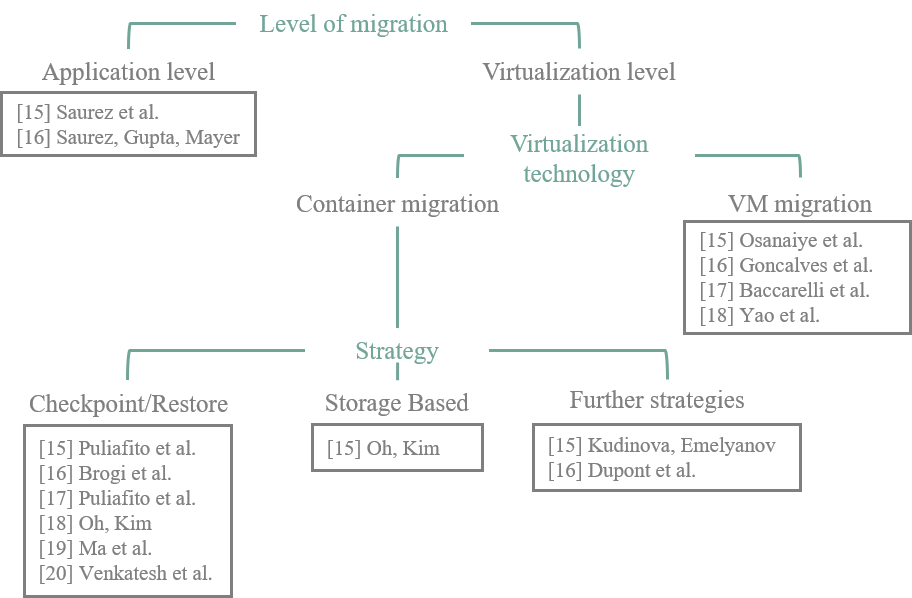
\includegraphics[width=\textwidth]{figures/visualizations/RelatedWorkFogOverview_1500.png}
\caption{Overview over related works regarding application migration in the fog}
\label{fOverviewLiteratureFog}
\end{figure}


\subsubsection{Migration of Virtual Machines}
\label{lMigrationVM}
Since the migration of \gls{vm}s has already been extensively studied in traditional cloud computing \cite{Yao.2015}, works with the subject of \gls{vm} migration in the fog mainly focus on the optimization of already established migration procedures for fog-specific use cases. Forsman et al. \cite{Forsman.2015} give an overview of the three general approaches for \gls{vm} migration. Cold migration shuts down the guest \gls{os} and moves it to a new host, where it is restarted. Hot migration does not shut down the guest \gls{os} but instead suspends it before moving it to another machine, where it is resumed. Hot migration thereby circumvents the termination of applications. Instead, they continue running on the new host. The third approach is the so-called live migration, which moves a \gls{vm} while it is still running on the original host. The downtime of applications migrated between fog nodes is thereby vastly reduced. Because of the reduced downtime, live migration is the preferred approach for \gls{vm} migration in the fog \cite{Baccarelli.2018, Osanaiye.2017}. Both Osanaiye et al. \cite{Osanaiye.2017} and Baccarelli et al. \cite{Baccarelli.2018} utilize so-called pre-copy live migration. Pre-copy live migration transfers memory contents in several iterations between the former and the new host \cite{Osanaiye.2017}. In contrast, post-copy live migration initially sends the whole virtual processing unit and the device state to the new host, allowing the new host to fetch memory pages on demand \cite{Osanaiye.2017}. While Osanaiye et al. \cite{Osanaiye.2017} focus on minimizing the downtime by evaluating whether to proceed with the stop and copy phase of the migration, Baccarelli et al. \cite{Baccarelli.2018} optimize the decision making process over the question if a \gls{vm} should be migrated, to ensure low energy consumption over wireless 5G connections.\\
The work of Yao et al. \cite{Yao.2015} also focuses on the decision if the migration is desirable, while at the same time deciding on an appropriate target node for the migration, optimizing the decision in terms of low overall network cost.\\
Lastly, Goncalves at al. \cite{Goncalves.2018} explore a simulation-based mobility prediction strategy to proactively migrate \gls{vm}s, with the intent of minimizing the latency. Using mobility prediction, they achieve a decrease in the number of performed migrations, resulting in a lower time of unavailability.


\subsubsection{Migration of Containers}
\label{lMigrationContainer}
As shown in Figure \ref{fOverviewLiteratureFog}, there are different approaches to the migration of containers. In \cite{Dupont.2017} the straight-forward solution of an orchestrated container destruction on the origin node, followed by container re-deployment on the target node, is proposed. This approach, however, does not allow the migration of stateful applications.\\
To allow the re-deployment of containers with their respective states, many authors concentrate on concepts exploiting \gls{criu}, which resembles the live migration approaches for \gls{vm}s mentioned before. \gls{criu} is a Linux software that can freeze, checkpoint, and restore running containers \cite{.29042020}. After an application's restoration, it resumes running precisely at the point it was frozen \cite{.29042020}. Puliafito et al. \cite{Puliafito.2019} conduct a detailed comparison of migration approaches that use \gls{criu}. The compared container migration techniques are mostly similar to the approaches for \gls{vm} migration. The first described possibility is cold migration, which they characterize as the iterative approach of stopping the container, dumping its state, transferring the dump to the target node, and resuming the container there. In contrast, they also describe live migration techniques, where the container keeps running while most of the state is transferred. Pre-copy, post-copy, and hybrid migration are differentiated. They all use multiple transfer steps reducing the downtime to a fraction of the total migration time. The pre-copy technique uses an initial pre-dump that is transferred to the target node. After transmission, the container on the origin node is stopped, and the modified state is dumped and transferred to the target node, where the container is resumed. In comparison, post-copy directly stops the container on the origin node but transfers only the minimal task state required to start the container \cite{.27112018}. After the transfer, the container is resumed on the target node, where it requests missing memory pages from the origin node whenever the resumed container tries to access memory pages that have not yet been transferred. Lastly, hybrid migration combines pre-copy and post-copy migration techniques. According to the authors' performance evaluation, the post-copy and the hybrid approach have a comparably low downtime. However, these approaches also suffer from a degraded service performance because of the necessity to request missing memory pages from the origin node. Additionally, failures during the migration are more severe since the up-to-date container state is distributed between the origin and the target node.\\
In practice, \cite{Brogi.2018} and \cite{Oh.2018} show the general possibility to migrate a container using \gls{criu}. Brogi et al. \cite{Brogi.2018} additionally point out that the integration of \gls{criu} into containerization technology can be a possible limitation. As of now, there are still compatibility issues between \gls{criu} and the containerization software Docker \cite{.27032020}, which highlights the actuality of the issue.\\
This is complemented by publications that introduce frameworks for the dynamic triggering of the migration. The authors of \cite{Puliafito.2018} propose a platform that monitors position and resource constraints. Based on these factors, the platform triggers a container migration via \gls{criu}.\\
Another focus of research is the improvement of the checkpoint and restore functionality itself. Ma et al. \cite{Ma.2019} approach the issue by leveraging the layered storage architecture of docker containers to reduce the transferred file systems size. Venkatesh et al. \cite{Venkatesh.2019} take a different approach. By avoiding expensive file system writes through the usage of Linux kernel support for multiple individual \gls{vas}, they get a modified \gls{vas}-\gls{criu} that stores memory snapshots in \gls{dram}, thereby vastly accelerating the snapshotting process.\\
An interesting work concerning container live migration is by Kudinova and Emalyanov \cite{Kudinova.2017}, who address the problem of faulty process states when the containers process tree is restored on the target node. They state that this problem can also occur when restoring from a checkpoint by using \gls{criu}. In their paper, they develop a mathematical model for the operation sequence needed to restore the process tree correctly.\\
Another approach to container migration presented by Oh and Kim \cite{Oh.2018} is the so-called storage-based migration. This approach uses a universally accessible storage volume on which the state of the origin container is stored. During the migration, the storage volume is detached from the origin node and attached to the target node, which uses the saved state on the persistent volume to restore the container's state after it is started. Since their paper focuses on the advantages of checkpoint-based migration (using \gls{criu}) over storage-based migration, they also point out the limitations of storage-based migration. In storage-based migration, the deployed containerized applications need to be prepared to save and restore the state. Additionally, this migration type comes with a heavy storage access dependency and high storage provisioning cost, limiting their usefulness in fog computing.


\subsubsection{Explicit State Management at Application-Level}
\label{lMigrationApplicationLevel}
Integrating explicit state management directly into deployed applications, the application level approaches fundamentally differ from the virtualization level approaches. Addressing the migration at application level allows specifically addressing application specific requirements at the expense of a less generalized solution.\\
In \cite{Saurez.2016} and \cite{Saurez.2017} the authors propose the programming infrastructure Foglets, which is aimed at geologically-distributed computing on fog and cloud nodes. Foglets allows for so-called Worker Processes, which execute the deployed applications computation, to be migrated between fog nodes. Each of the Workers running on a node implement two handlers that expose the state of the Worker. The first handler captures the volatile state on the origin node and assures that related computations are completed and saved. The second handler uses this volatile state as input to initialize the local state of the target node. Simultaneously with the execution of these two handlers, persistent data, stored in a RocksDB database, is migrated to the target node. These inner-workings of Foglets are outlined in the first publication of Saurez et al. \cite{Saurez.2016}. In a follow-up publication on Foglets \cite{Saurez.2017} the authors demonstrate Foglets capability to migrate a stream-processing application's state across nodes, supported by contextual information.

\subsection{State in Data Processing}
\label{lStateDataProcessing}
The second category of related works considered in this thesis are publications looking at the role of state in data- and, more specifically, stream-processing. The considered works are further categorized in Figure \ref{fOverviewLiteratureState}. While there are fundamental works that look at the grand topic of state management, most others focus on the actual usage of state in their respective systems. In these publications, state is used in migration, for fault tolerance and/or for system scalability. Additionally, the paper of Ouyang et al. \cite{Ouyang.2011} follows an entirely different approach and therefore has to be distinctly classified.\par


\begin{figure}[H]
\graphicspath{{./figures/code/}}
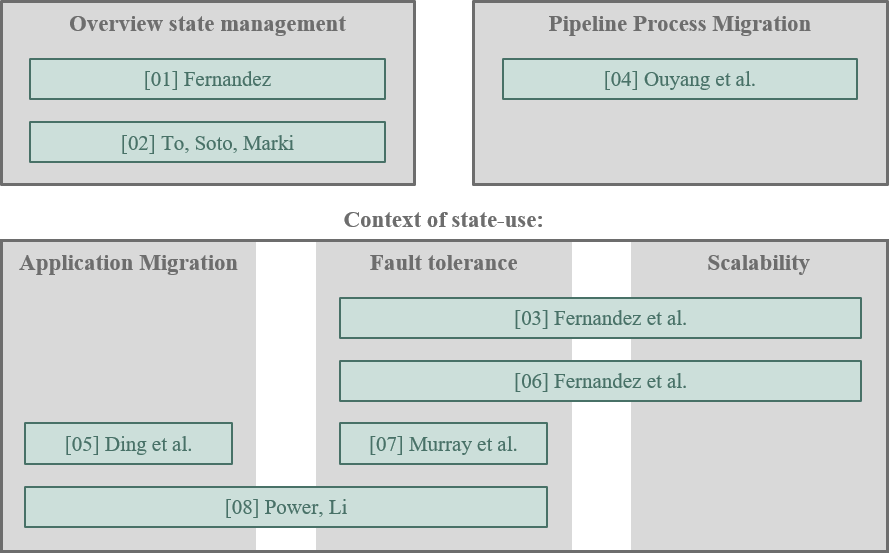
\includegraphics[width=\textwidth]{figures/visualizations/RelatedWorksStateManagement_1500.png}
\caption{Overview over related works regarding state in data processing}
\label{fOverviewLiteratureState}
\end{figure}

In \cite{CastroFernandez.2016} and \cite{To.2017} state management is investigated on a general level. While \cite{To.2017} surveys state management in big data systems, \cite{CastroFernandez.2016} addresses insufficient state management as the main shortcoming of modern data-parallel processing systems, therefore diving deeply into the issue of state.\\
One operation that requires the correct management of an application's state is scaling. Scaling refers to the parallelization on operator level to improve throughput in computationally expensive operators to avoid bottlenecks \cite{CastroFernandez.2013}. Fernandez et al. \cite{CastroFernandez.2013} enable scaling by exposing the processing state. They model the processing state as a set of key/value pairs. To expose the state, developers have to implement a get-function for each developed operator, locking all internal data structures while taking a copy of them. In addition to scaling, the publication focuses on fault tolerance. Fault tolerance means the capability to recover from faults that occur during the application's execution. The authors achieve fault tolerance by asynchronously checkpointing the operator state of the operators to upstream nodes. These checkpoints are used to restore failed operators by setting the processing state, with the help of a developer implemented set-function. After the processing state is restored, unprocessed events are replayed from the buffer state, resulting in an up-to-date processing state. The same authors also published another paper \cite{Gibson.2014} taking a similar approach to achieve fault tolerance and scalability. In this work, they once again use asynchronous checkpointing. Furthermore, they minimize the disruption in processing during checkpointing by using so-called dirty state. The dirty state of a \gls{pe} is acquired by checkpointing a \gls{pe} while it continues processing events. In addition, they propose a concept for distributing state between processing nodes.\\
In contrast to this asynchronous checkpointing tactic, other authors utilize synchronous global checkpointing using a "stop-the-world" approach \cite{Murray.2013} and asynchronous global checkpointing using the Chandy-Lamport algorithm \cite{Chandy.1985, Power.2010} to provide checkpoints for fault-tolerance.\\
The third context in which state is used in related publications, is for the migration of \gls{pe}s. Ding et al. \cite{Ding.15012015} propose a migration mechanism that performs a progressive migration of the operator state. It allows processing while the operator state is migrated, achieving a reduction in downtime. Furthermore, they outline challenges arising due to the migration. They identify the impossibility of parallely executing and migrating a task, the possibility that the origin node might still receive inputs after the migration, and issues in the transmission of operator states as main challenges. In comparison to this work, the authors of \cite{Power.2010} base their migration concept on shared and distributed state. This makes the migration of data processing applications trivial since a consistent state is prevalent at all nodes. However, this design comes at the expense of high networking and computation costs since all changes to the operator state need to be committed \cite{Ding.15012015}, hindering the usefulness in fog infrastructures.\\
In contrast to these approaches, Ouyang et al. \cite{Ouyang.2011} follow a similar concept for the acquisition of the state to the checkpoint/restore container migration approaches presented in chapter \ref{lMigrationContainer}. However, while in these approaches, the whole container with its running applications is migrated, in \cite{Ouyang.2011}, only the processes, which comprise the application, are migrated by using \gls{blcr}. \gls{blcr} is a tool that can create checkpoints of running processes and can restart the processes from the checkpoints. Firstly, all processes are suspended and checkpointed, then the process images containing the checkpoints are transferred to the migration target node, where they are then restarted and reconnected to a stream processing pipeline. While this approach shares many characteristics of the checkpoint/restore container approaches, it performs the checkpointing and restoring actions on the application level, instead of the virtualization level. This makes the approach more versatile since singular processes can be migrated. The authors achieve a significant performance improvement by utilizing remote direct memory access, which reduces networking overhead and data \gls{io}. Requiring a an InfiniBand connection between nodes makes the approach proposed by the authors a poor fit for the fog infrastructure.

\subsection{Research Gap}
\label{lResearchGap}

Table \ref{tComprehensiveOverview} gives a comprehensive overview of the approaches presented in the related work. Using this overview, the research gap can be conclusively outlined.\\
Altogether, the works regarding the migration of applications in the fog do not sufficiently address stream processing. In addition, they solely focus on the migration of correctly running applications, neither providing a possibility to migrate a faulty application nor proposing any measures to provide fault tolerance.\\
On the other hand, approaches from the "state in data processing" field do not address fog computing specific requirements.\\
Out of the twelve compared works only three (\cite{Puliafito.2018, Oh.2018, Ding.15012015}) publications mainly focus on the migration process. This lack in research is also pointed out by Ding et al. \cite{Ding.15012015}, stating that other works often lack a precise description of the used migration tactics.\\
Moving forward, this thesis thus should fill these gaps, by proposing an extensive conceptual framework for the adaptation of stream processing pipelines in fog infrastructures. While doing so, the contents of the migration and the exact procedure should be described in detail.

\newcommand*\rot{\rotatebox{90}}
\newcolumntype{P}[1]{>{\centering\arraybackslash}p{#1}}

\begin{table}[H]
    \caption{Comprehensive overview of related work}
    \label{tComprehensiveOverview}
    \centering
    \begin{tabular}{|p{2cm}|P{0.5cm}|P{0.5cm}|P{0.5cm}|P{2.5cm}|P{2.5cm}|P{2cm}|P{2.5cm}|}
    \hline
     \rot{\textbf{Publication}} & \rot{\textbf{Migration}} & \rot{\textbf{Fog Considerations}} & \rot{\textbf{Fault Tolerance}} & \rot{\parbox{2cm}{\textbf{State \\Abstraction}}} & \rot{\parbox{2cm}{\textbf{Checkpointing \\Mechanism}}} & \rot{\textbf{Intended Use}} & \rot{\parbox{3cm}{\textbf{Main Focus \\of Publication}}}\\ 
     \hline
     Baccarelli et al. \cite{Baccarelli.2018} & \checkmark & \checkmark & \ding{55} & \gls{vm} checkpoint & \gls{vm} checkpointing & general & optimize energy usage\\
     \hline
     Osanaiye et al. \cite{Osanaiye.2017} & \checkmark & \checkmark & \ding{55} & \gls{vm} checkpoint & \gls{vm} checkpointing & general & optimize migration\\
     \hline
     Puliafito et al. \cite{Puliafito.2018} & \checkmark & \checkmark & \ding{55} & container checkpoint & \gls{criu} & general & migration\\
     \hline
     Brogi et al. \cite{Brogi.2018} & \checkmark & \checkmark & \ding{55} & container checkpoint & \gls{criu} & stream processing & fog node management\\
     \hline
     Oh, Kim \cite{Oh.2018} & \checkmark & \textasciitilde & \ding{55} & container checkpoint & \gls{criu} & general & migration\\
     \hline
     Ma et al. \cite{Ma.2019} & \checkmark & \textasciitilde & \ding{55} & optimized container checkpoint & top level container storage & general & optimize migration\\
     \hline
     Dupont et al. \cite{Dupont.2017} & \textasciitilde & \textasciitilde & \ding{55} & - & - & \gls{iot} functions & orchestration\\
     \hline
     Saurez et al. \cite{Saurez.2016} & \checkmark & \checkmark & \ding{55} & operator state & interface in application & general & orchestration\\
     \hline
     Ouyang et al. \cite{Ouyang.2011} & \checkmark & \ding{55} & \ding{55} & process checkpoint & \gls{blcr} & stream processing & optimize migration\\
     \hline
     Ding et al. \cite{Ding.15012015} & \checkmark & \ding{55} & \ding{55} & operator state & interface in application & stream processing & migration\\
     \hline
     Murray et al. \cite{Murray.2013} & \ding{55} & \ding{55} & \checkmark & shared global state & interface in application & stream processing & orchestration\\
     \hline
     Power, Li \cite{Power.2010} & \checkmark & \ding{55} & \checkmark & shared global state & Chandy-Lamport & data processing & orchestration\\
     \hline
     Fernandez et al. \cite{CastroFernandez.2013} & \ding{55} & \ding{55} & \checkmark & operator state & interface in application & stream processing & fault tolerance\\
     \hline
     \textit{This Thesis}& \checkmark & \checkmark & \checkmark & \textit{operator state} & \textit{interface in application} & \textit{stream processing} & \textit{migration}\\
     \hline
    \end{tabular}
\end{table}